\section{Results} \label{sec:3}
The final results for the $v_{2}$ elliptic flow coefficient were obtained using the method in (\ref{subsec:2.2}) and was processed and visualized using the ROOT library.

\begin{figure}[h]
	\centering
	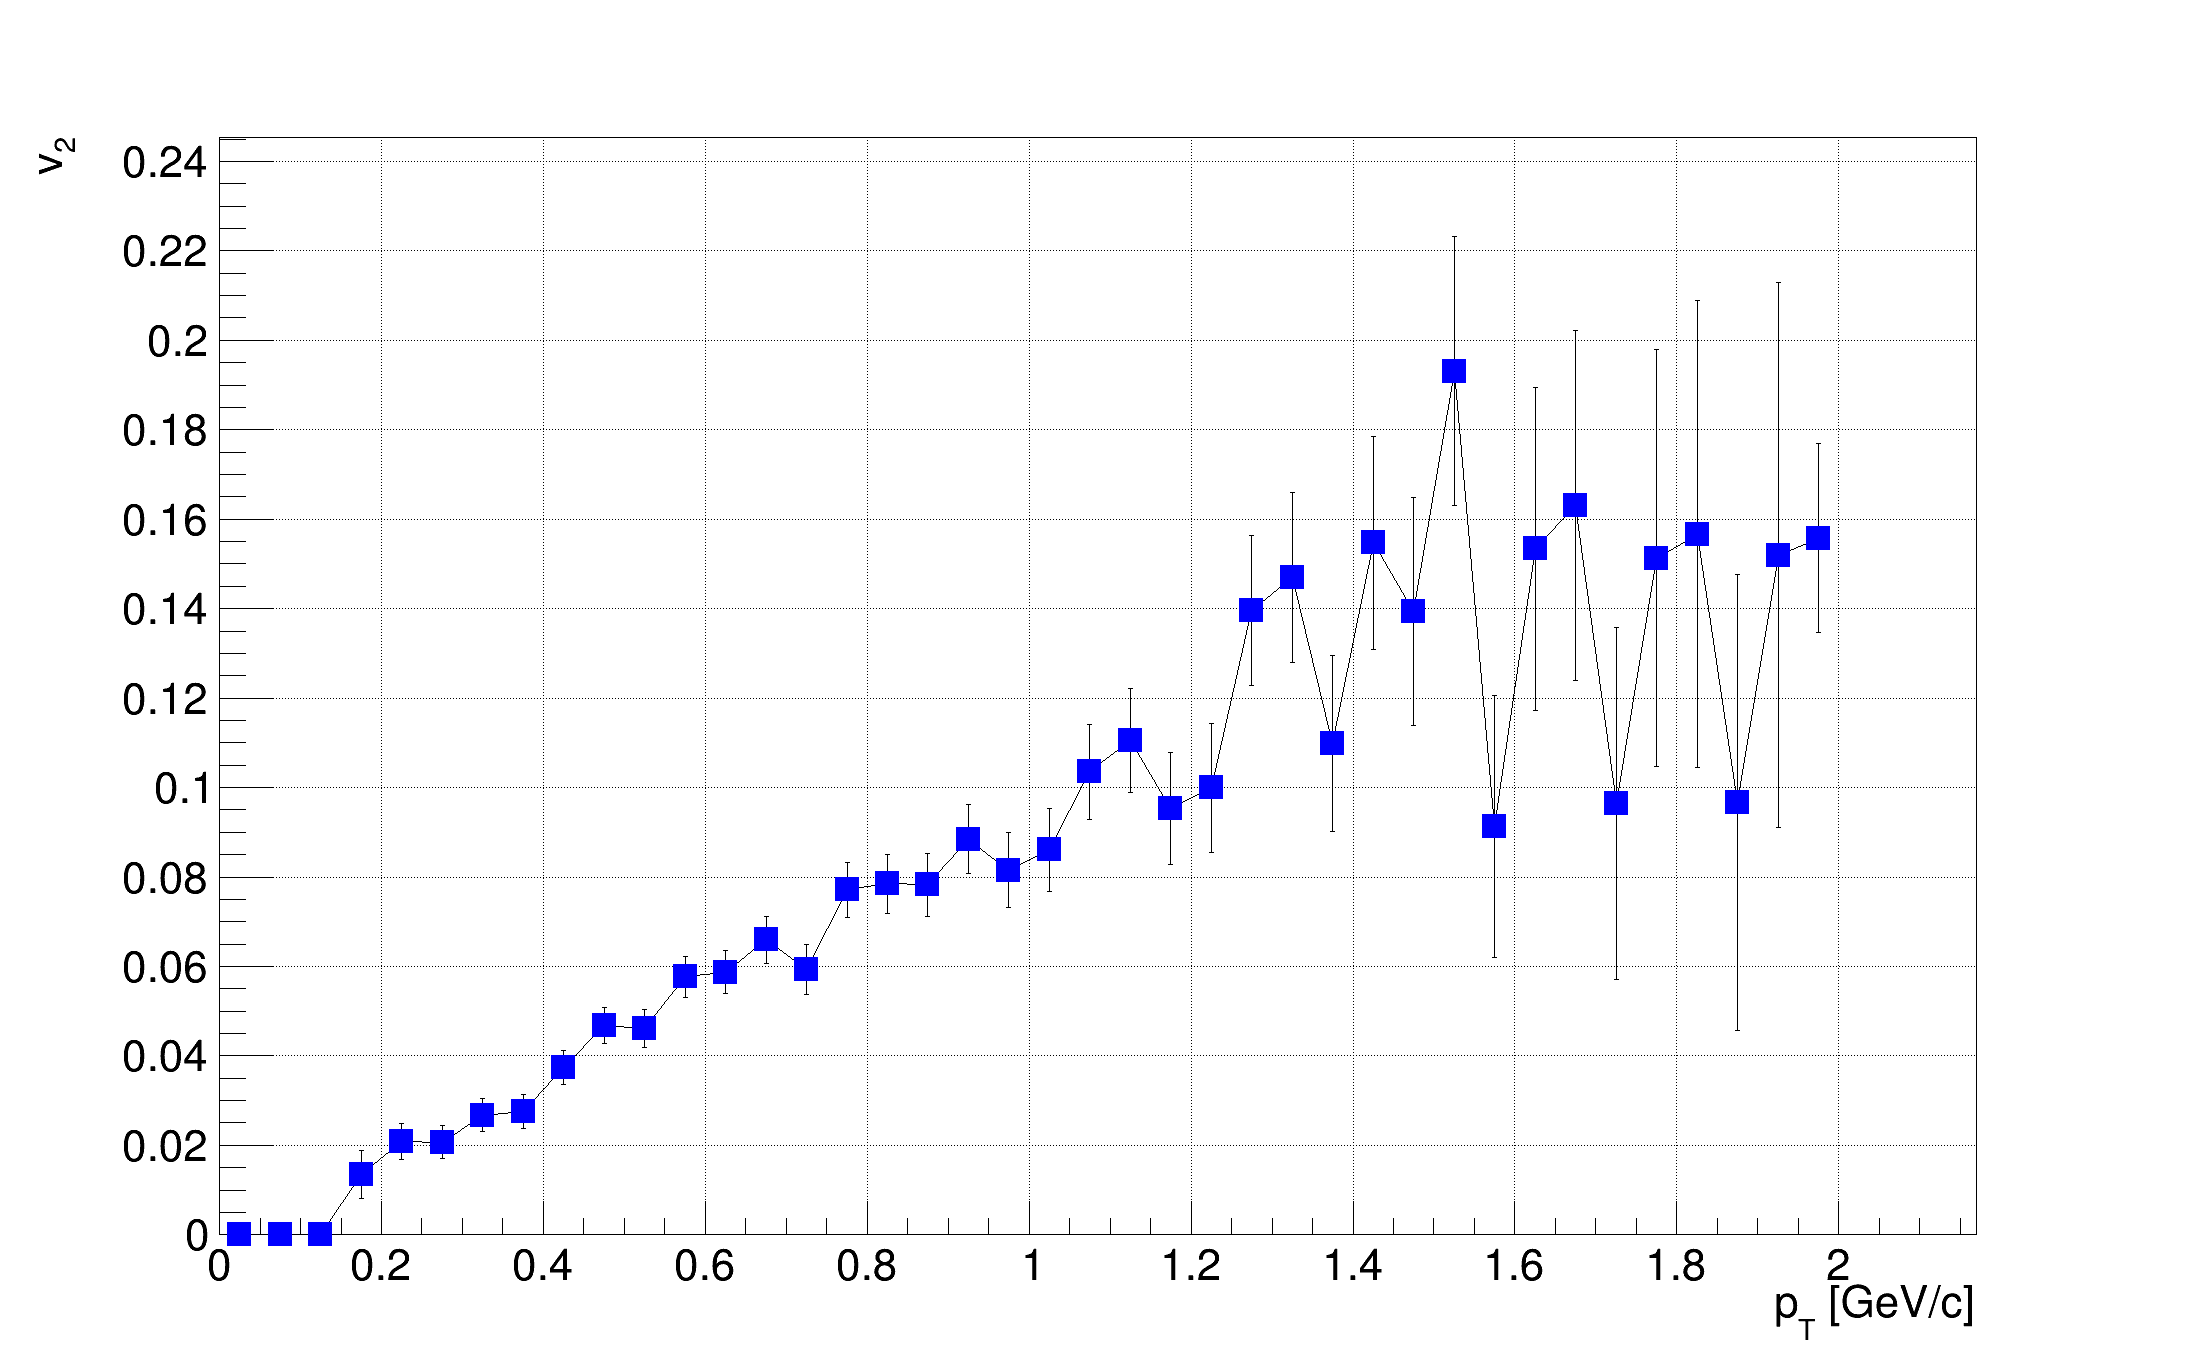
\includegraphics[width=0.8\textwidth]{v2_flow_per_pt.png}
	\captionof{figure}{The $v_{2}$ elliptic flow coefficient as a function of the $p_{T}$ transverse momentum for a single centrality class of $0\% - 92\%$.}\label{fig:4}
\end{figure}

For this numerous literature can be cited eg. Fig. (2) in \citep{Collaboration2003} -- as it was already mentioned here. This figure can be seen on Fig. (\ref{fig:5}) here in this paper. The very same characteristics can be observed on the obtained results in Fig. (\ref{fig:3}) and in Fig. (\ref{fig:5}). One of them that can be seen on both figures is that the $p_{T} - v_{2}$ curve saturates as it reaches $p_{T} \approx 1$ or $2\ \mathrm{GeV}/\mathrm{c}$, just like as it is mentioned in eg. \citep{Collaboration2003} or \citep{Retiere2004}. The maximum value of $v_{2}$ is approximately $0.25$, but the large errors in the high $p_{T}$ regime makes it impossible to estimate it more precisely. Nonetheless this value is close to the ones on Fig. (\ref{fig:5}), where $v_{2} \left( p_{T} = 2\ \mathrm{GeV}/\mathrm{c} \right) \approx 0.16$. The difference can be attributed to the wide centrality class used to calculate the $R$ event plane resolution factor on.

\begin{figure}[h]
	\centering
	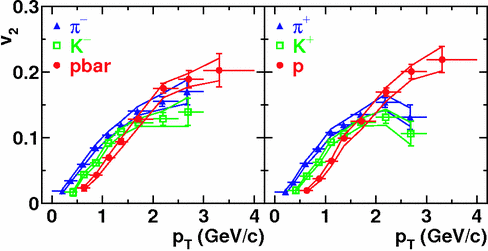
\includegraphics[width=0.6\textwidth]{cite.png}
	\captionof{figure}{The two upper panels of Fig. (2) from \citep{Collaboration2003}. The relevant lines here are those that belong to the pion measurements.}\label{fig:5}
\end{figure}

At the end I've obtained results consistent with values in the literature, which implies that the calculations here were probably correct. The errors of the $v_{2}$ values could be probably improved by choosing a more robust fitting method for the angle distribution, but it probably won't change the final implications of the results.